\documentclass{IEEEtran}

\usepackage{lettrine}
\usepackage{placeins}
\usepackage{authblk}
\usepackage{tabularx}
\usepackage{graphicx}
\usepackage[strings]{underscore}
\usepackage[normalem]{ulem}
\usepackage{float}
\usepackage{caption}
\useunder{\uline}{\ul}{}

\DeclareUnicodeCharacter{200A}{} 

\begin{document}

    \title{Deep Neural Network with Raspberry Pi}


    \author{
        \IEEEauthorblockN{Lauro Cabral and Sotheanith Sok\\}
        \IEEEauthorblockA{California State University, Long Beach\\ Email: \{lauro.cabral, sotheanith.sok\}@student.csulb.edu}
    }
    \date{October 17 2020}
    \maketitle

    \begin{abstract}
        As the price of GPUs continues to increase, it has become increasingly difficult for average consumers to obtain the necessary hardware for experimenting with neural networks at home. Fortunately, it is possible to train a neural network through other means and this paper aims to explore the possibility of using distributed systems to do so. By combining dask, a highly efficient library for parallel computing, and raspberry pi, a relatively cheap single-board computer, it is possible to create a cluster of nodes that is fairly efficient at solving deep learning problems and with a high degree of scalability. Additionally, such a setup is also beneficial in terms of hardware flexibility as any raspberry pi node can be replaced with other hardware including an Intel-based system and an AMD-based system without sacrificing the performance. Lastly, by using dask as the backend library, the current setup can be adapted to work with many popular deep learning libraries including Tensorflow and Scikit-learn with minimal code modification while maintaining a similar result.
        \end{abstract}

    \section{Introduction}
        \IEEEPARstart{I}n the last few years, the deep learning field has seen tremendous advancement that enables the creation of many life-changing technologies including autonomous driving, self-taught AI, and pattern recognition. This progress is only possible due to the availability of high-performance GPUs which excel at solving multiple floating pointing problems simultaneously.
        According to PassMark Software, a crowd-sourced GPU benchmark database, the current flagship GPU is approximately twenty-five thousand timers faster than the flagship GPU from 20 years ago \cite{passmark_software}. 

        \begin{figure}[!htb]
            \centering
            \captionsetup{justification=centering}
            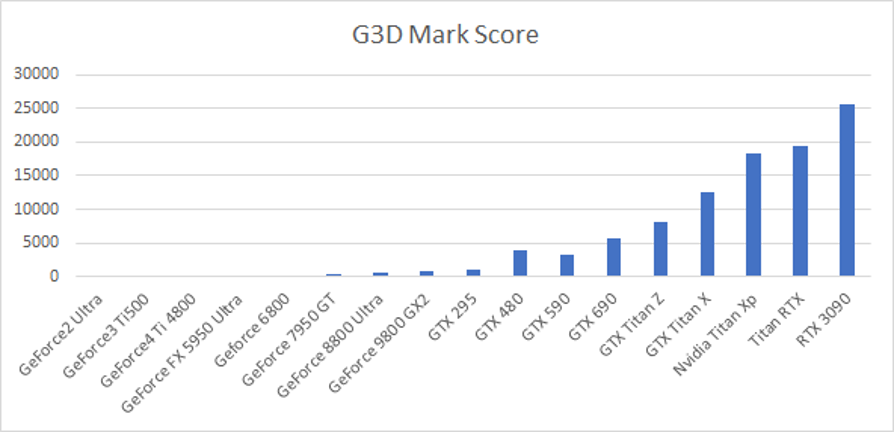
\includegraphics[width=\linewidth]{GPU_Improvment.png}
            \caption{Generational improvement of Nvidia flagship GPU}  
        \end{figure}
        
        Unfortunately, as the interest in the deep learning field increases, so did the demand for high-performance flagship GPU and as such, the price of flagship GPU has increased exponentially. Today, the high-end flagship GPU is 4 times as expensive as the flagship GPU from 20 years ago \cite{passmark_software} and this price increase makes it difficult for average consumers to obtain necessary hardware for experimenting with the deep neural network at home. As such, this paper is intended to explore the possibility of using a distributed system of relatively cheap hardware to solve a deep learning problem. This paper will start by covering the history of deep learning including its initial hurdles, its rise, and the current obstacles. Then, the paper provides an overview of how deep learning works such as forward propagation and backward propagation and techniques for parallelizing deep learning problems. Furthermore, this paper will discuss the implementation of one of the parallelization techniques as well as its setup, advantages, and limitations. Finally, the last part of the paper will contain recommendations and discussions on future works.

        \begin{figure}[!htb]
            \centering
            \captionsetup{justification=centering}
            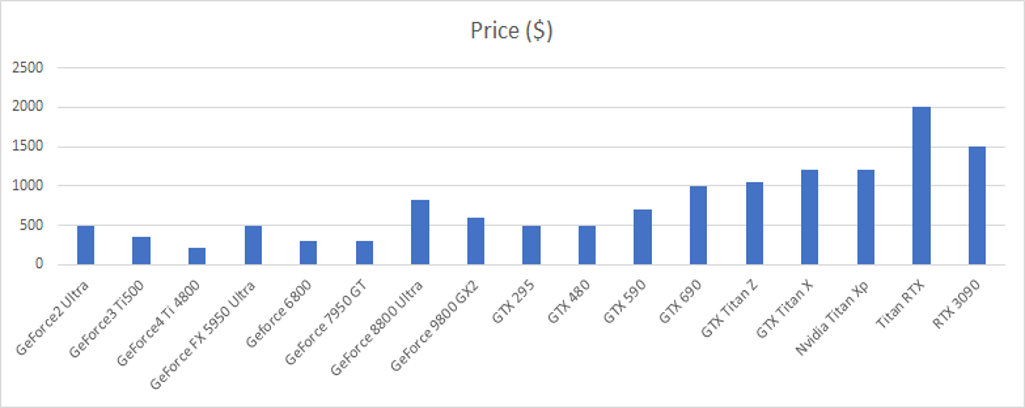
\includegraphics[width=\linewidth]{GPU_Price.png}
            \caption{MSRP of Nvidia flagship GPU}  
        \end{figure}

    
    \section{History of Deep Learning}
        Since its initial conception in 1967 by Alexey Ivakhnenko, two major hurdles of applying deep neural networks in solving real-life problems are hardware limitations and data limitations. To start with, a majority of hardware designed at that time was focused on single-core performance because that is what a majority of applications required \cite{inproceedings}. Thus, there was no incentive for developing hardware that has more than a single core. Unfortunately, this single core focus hardware is terrible for solving neural network problems because each node in a layer has to be calculated linearly before it can proceed to the next layer. Second, since the internet wasn’t widespread at the time, any dataset that needed to train a neural network would need to be collected manually \cite{pew_research_center}. This process is prohibitively expensive and thus, good datasets are hard to come by. This hardware restriction and data constraint stifled any advancement in the field for many years to come.

        \begin{figure}[!htb]
            \centering
            \captionsetup{justification=centering}
            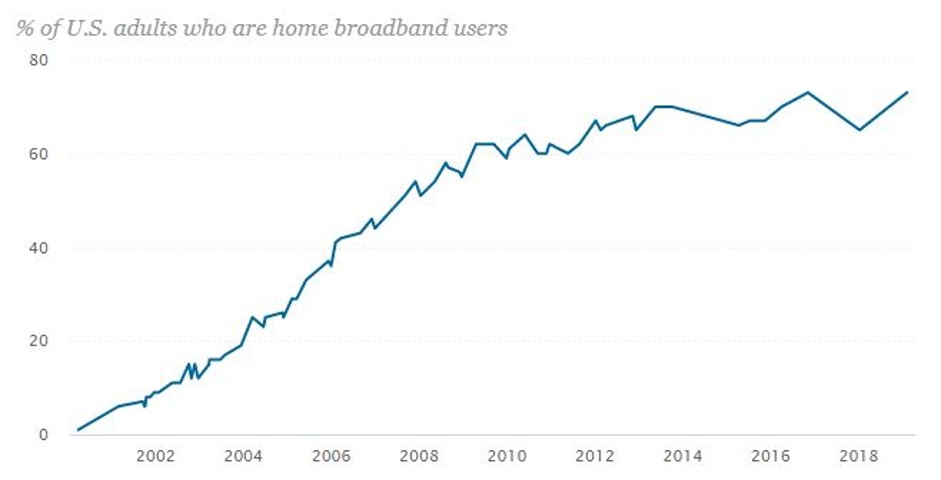
\includegraphics[width=\linewidth]{USBroadband.png}
            \caption{Percent of U.S. adult who are home braodband users}  
        \end{figure}

        The rise of deep learning, in the last few years, is the result of the widespread availability of high-performance GPU which was primarily designed for rendering complex and dynamic scenes in real-time \cite{nickolls_dally_2010}. Interestingly, rendering dynamic scenes and training neural networks require similar forms of hardware solutions which compose of many fast floating-point calculating cores. Furthermore, with the rise of the internet and the way people interact with it, it has become easier and cheaper than ever to collect a massive amount of datasets \cite{deng_dong_socher_li_li_fei-fei_2009}. These two factors fuel the deep learning revolution that occurs today and neural networks are being adapted to solve problems that were considered too complicated for a computer to solve.
        
        However, as the deep learning field continues to make massive progress, a new problem is rearing its heads and threatening the potential growth of the field. Today, the general conscience on how to improve a neural network is to make it wider and deeper which, in theory, should increase the network representative power. And, as the network gets more complications, it also requires more datasets to train properly. As a result, the current state of the art neural networks is composed of hundreds of nodes and layers and require millions of datasets to train. This exponential increase in the volume of information means that neural networks of today have outgrown the information capacity of most modern hardware. To simply put it, neural networks are getting too large for a majority of GPU to represent and its training datasets are too big for most computers to store in their memories \cite{ben-nun_hoefler_2019}. To address the hardware restriction described above, many researchers have turned to the distributed system as a possible solution. The common setup for such a system is a cluster of one to many computers where each computer has as many GPUs as the computer's PCI-E bandwidth allows which is around two to four.  Even though such a setup has shown promising results, its cost is undoubtedly high and as such, it will be a great barrier of entry for most consumers which, ultimately, could harm the future growth of deep learning as a field.
        
    \section{Deep Learning Basic}
        At its fundamental idea, a deep neural network is a universal approximator which means that it can reproduce any function by observing at said function inputs and outputs. Deep neural networks can accomplish this because of its structure which consists of multiple layers of neurons, weights, and biases \cite{hornik_1991}. For a neural network to approximate any function, it first needs to go through a training process where its weights need to be adjusted based on how accurate its predicted output is compared to the true outputs. This training process consists of two distinct phases: forward propagation and backward propagation. 

        \begin{figure}[!htb]
            \centering
            \captionsetup{justification=centering}
            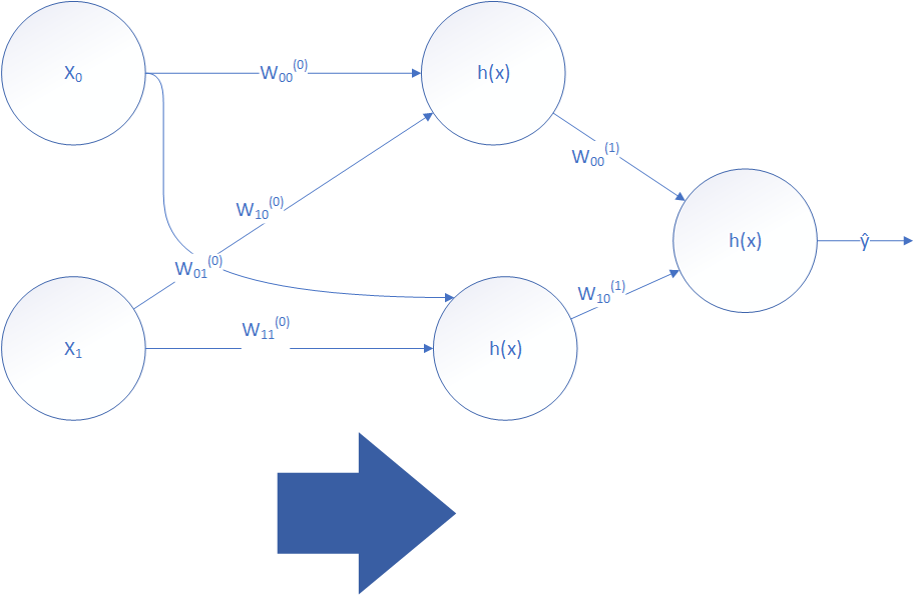
\includegraphics[width=\linewidth]{ForwardProp.png}
            \caption{Forward Propagation: Inputs flow from left to right}  
        \end{figure}

        To start with, the main purpose of the forward propagation phase is to see what kind of outputs are produced by a network given some inputs. This process starts by feeding inputs into the first layer and forwards outputs from such layers to the next layers. Inside the layer, neurons are responsible for taking outputs of previous layer neurons and multiplying them with their respective connection weights. Then, the neuron accumulates the resulting values and passes the sum into some kind of activation function to produce the output for this neuron. It is worth noting that the activation function is necessary for deep neural networks in order to introduce some form of nonlinearity into the network which will enable the network to approximate nonlinear function \cite{luhaniwal_2020}. This process of passing outputs from one layer to the next is repeated until the final output is achieved.

        \begin{figure}[!htb]
            \centering
            \captionsetup{justification=centering}
            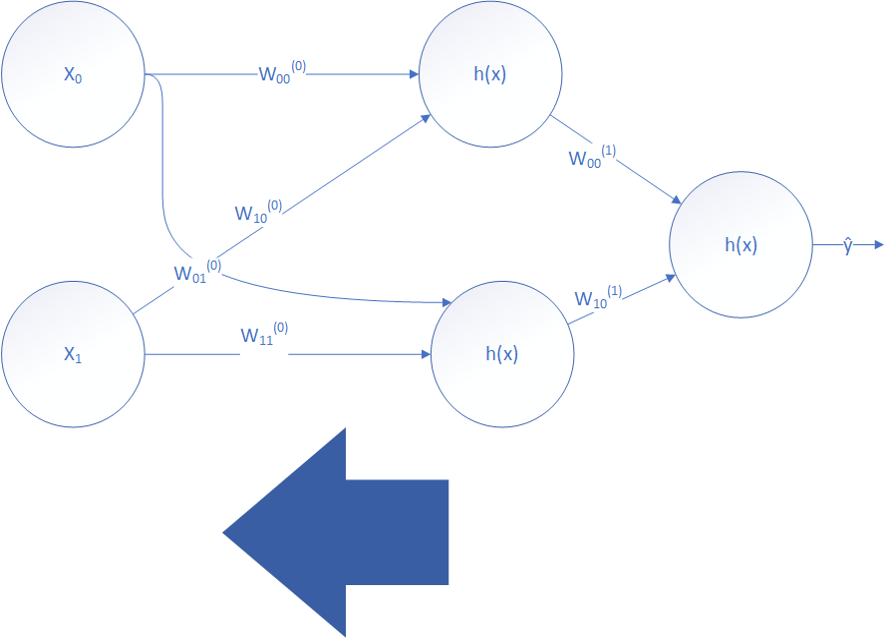
\includegraphics[width=\linewidth]{BackwardProp.png}
            \caption{Back Propagation: Loss flows from right to left}  
        \end{figure}

        Initially, predicted outputs produced by the network will be wildly inaccurate when compared to the expected outputs because weights are randomly generated. However, those inaccuracies or errors do offer a hint on how to adjust the network’s weights to improve its performance. The main objective of the backward propagation phase is to adjust the network’s weights such that its errors are minimized and it accomplishes this with the help of the gradient descent algorithm. First off, predicted outputs and expected outputs are compared to produce an error value called loss. Then, the loss value is propagated backward throughout the network where, at each layer, gradient, or amount in which each weight contributed to the loss value gets calculated. Finally, each weight gets adjusted with their respective gradient and the entire process repeats itself until the loss is minimized \cite{kostadinov_2019}.

        At first glance, once would assume that the process of forward propagation and backward propagation are repeated for each pair of input and output and that would produce a well-trained network but it is not necessarily the case \cite{ruder2017overview}. The major problem that arises from adjusting weights for every dataset is the instability that would be introduced into the network which increases the chance of the network to converge on a suboptimal solution. Thus, it is recommended to train a network in batches of datasets which entails performing forward propagation steps for multiple datasets, average their losses, and use the average loss to perform backward propagation. 

    \section{Parallelization of Deep Learning}
        The consensus on how to deal with neural networks requiring more resources than what modern hardware can provide is through the use of distributed systems. However, in order for neural networks to be able to run on a distributed system, its structure needs to be changed. Currently, there are two types of parallelization that are recommended for a neural network and they are model parallelization and data parallelization.

        \begin{figure}[!htb]
            \centering
            \captionsetup{justification=centering}
            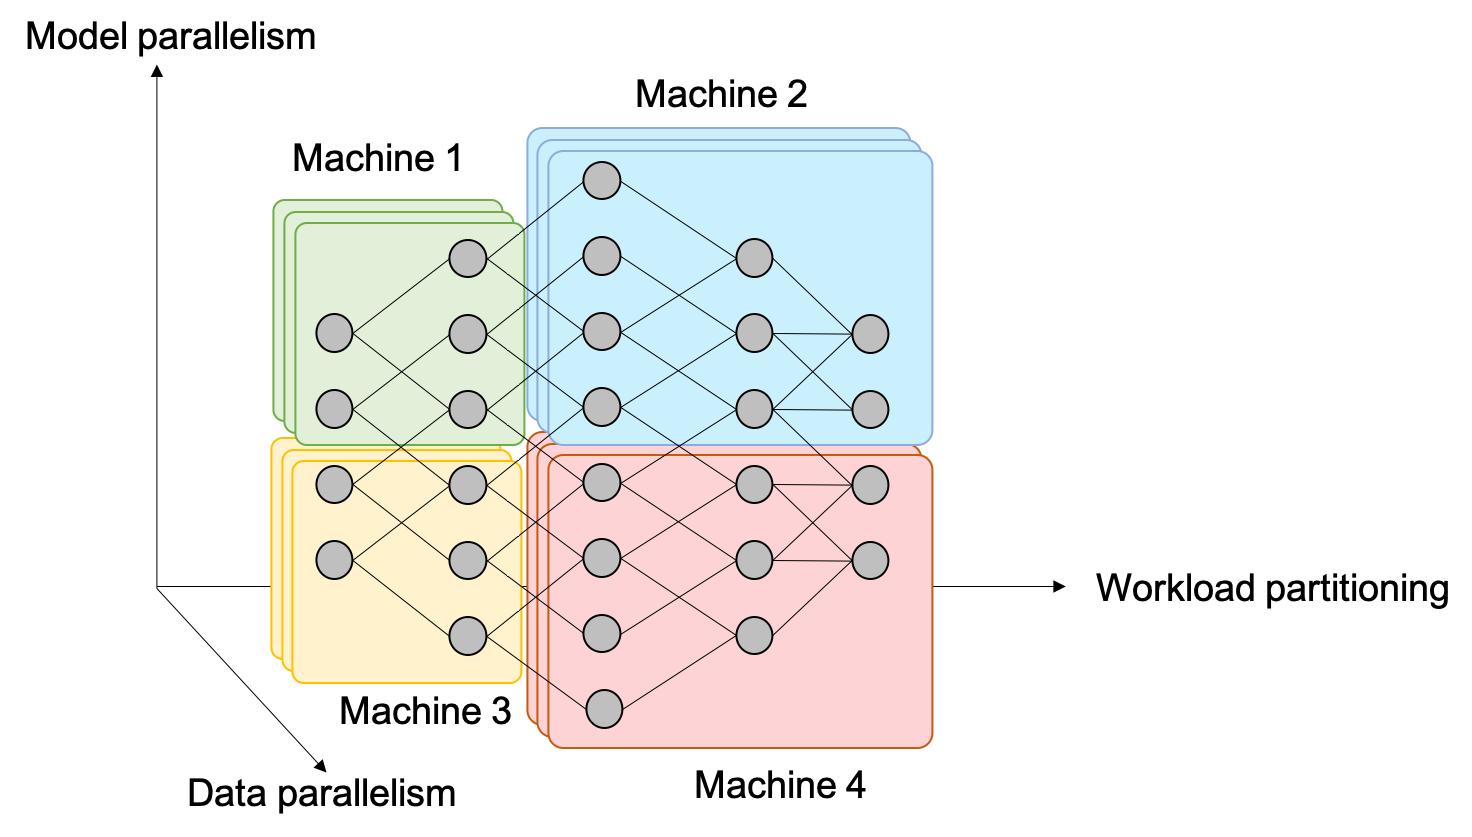
\includegraphics[width=\linewidth]{Parallelism.png}
            \caption{Model Parallelism vs Data Parallelism \cite{ekanayake}}  
        \end{figure}

        To start with, as network networks get more complicated, its hardware requirement is also increased. Thus, the goal of model parallelization is to address the scenario where networks are too deep or twice to be represented in a single GPU. This methodology calls for the slicing of networks into smaller groups of layers where each layer chuck can be loaded onto a separate GPU. Then, the training process occurs similarly to how a network gets trained on a single GPU but instead of passing values from one layer to another, values are passed from one GPU to another GPU \cite{ben-nun_hoefler_2019}.

        Unfortunately, as neural network complexity increases, the amount of datasets required to train such a network also increases exponentially which usually exceeds the capability of most computers to hold. As such, data parallelization aims to address this issue by splitting datasets into small chunks and distributing them onto multiple nodes. Then, each node processes its chunk of datasets independently and forward the average loss to either a central node for centralized architecture or the next node for map-reduce architecture. Finally, the accumulated loss gets averaged out based on the number of nodes in the cluster and the averaged loss gets propagated back onto all nodes where their weights get adjusted by their respective gradient \cite{ben-nun_hoefler_2019}.

    \section{Setup}
        In this experiment, software and hardware have been chosen such that it maximizes performance, flexibility, and ease of use while minimizes cost. 
        
        \begin{figure}[!htb]
            \centering
            \captionsetup{justification=centering}
            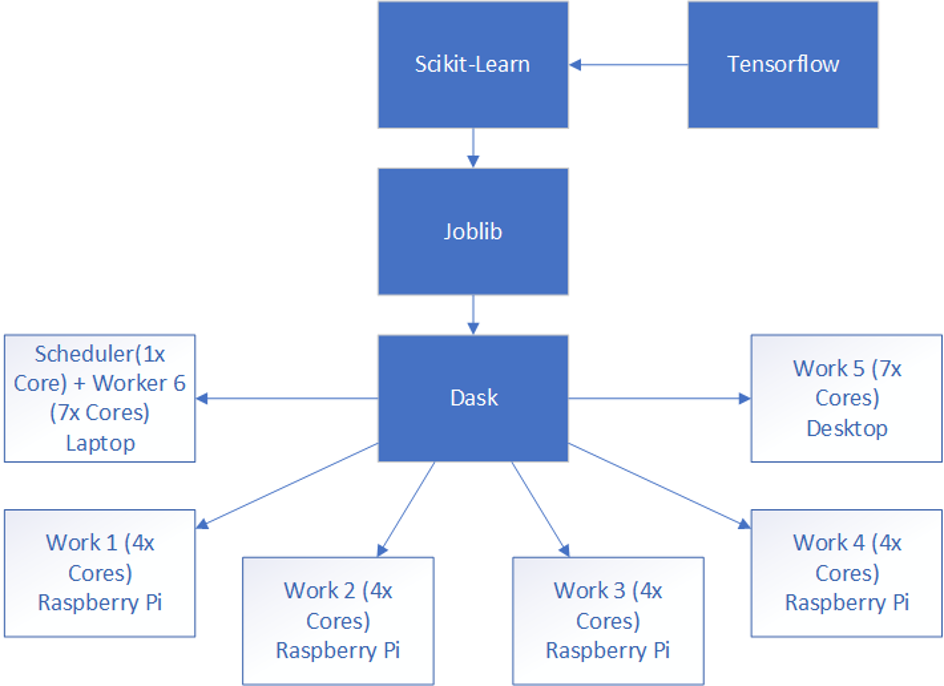
\includegraphics[width=\linewidth]{Stack.png}
            \caption{Hardware and software stack}  
        \end{figure}
            
        To start with, the hardware stack consists of four raspberry pi, one laptop, one desktop, and one consumer-grade router. All nodes are connected to the router with ethernet cables in order to limit the inter-node communication latency. First off, the desktop and the laptop contribute seven computing cores and ten gigabytes of memories each to the cluster while the desktop also provides a single core as the scheduler. Then there are four raspberry pi which contribute four computing cores and two gigabytes of memories each to the cluster. In total, the cluster will have up to thirty computing cores and thirty gigabytes of memories.

        \begin{table*}[]
            \begin{tabular}{|l|l|l|l|l|}
            \hline
            {\ul \textbf{Hardware}}                   & {\ul \textbf{Cores Count}} & {\ul \textbf{Ideal Execution Time (seconds)}} & {\ul \textbf{Measured Execution Time (seconds)}} & {\ul \textbf{Scalability}} \\ \hline
            1 x Raspberry Pi                          & 4                          & 901                                           & 901                                              & 1                          \\ \hline
            1 x Raspberry Pi, 1 x Desktop             & 11                         & 327.6363636                                   & 237                                              & 1.382431914                \\ \hline
            2 x Raspberry Pi, 1 x Desktop             & 15                         & 240.2666667                                   & 181                                              & 1.327440147                \\ \hline
            3 x Raspberry Pi, 1 x Desktop             & 19                         & 189.6842105                                   & 152                                              & 1.247922438                \\ \hline
            4 x Raspberry Pi, 1 x Desktop             & 23                         & 156.6956522                                   & 134                                              & 1.169370539                \\ \hline
            4 x Raspberry Pi, 1 x Desktop, 1 x Laptop & 30                         & 120.1333333                                   & 124                                              & 0.968817204                \\ \hline
            \end{tabular}
            \caption{Ideal execution time vs actual execution time for clusters training Random Forest Classifier}
        \end{table*}
        
        For the software stack, the choice of libraries is determined by the programming language and the availability and the maturity of libraries for implementing deep learning problems. The language of choice for this software stack is Python because of its simplicity and ease of use and the availability of many popular and mature libraries such as NumPy, Scikit-Learn, Panda, and Tensorflow which streamline the implementation of many modern deep learning models. Since Python is the language of choice, the obvious pick of distributed system management library is Dask which is a popular open-source library for parallel computing written purely in Python. In addition, Dask also provides native support for running a deep learning model on a cluster with the help of Dask-ML and JobLib libraries which act as middlewares between Dask and Scikit-Learn. 

    \section{Results}   

        For any experiment, it is important to establish a baseline result such that any subsequent results can be measured relatively to it. Thus, a single raspberry pi is used to train a Random Forest Classifier which will act as the baseline result and it takes the raspberry pi 901 seconds to complete the execution. This result is expected since the four computing cores of raspberry pi are relatively slow compares to modern computing cores. 
            
        Next, by combining computing cores of a raspberry pi and the desktop, the cluster's computing cores increases to 11 and it takes this cluster 237 seconds to train the Random Forest Classifier which translates to 138\% cores scaling efficiency. The abnormally high scaling efficiency is caused by the scheduler able to take full advantage of hardware heterogeneity and allocate more works to faster computing cores of the desktop. Increasing computing cores by adding more hardware to the cluster results in further improvements to the execution time at the cost of scaling efficiency across all cores. At 30 computing cores, the cluster is able to train the Random Forest Classifier in 124 seconds but it only achieves 97\% scaling efficiency. 
        
        There are multiple reasons that could explain the drop in scaling efficiency as cores count increases and one of those reasons is network latency. To simply put, as more hardware gets connected to the router, it will take that router longer to communicate from one hardware to another and this network latency scales linearly with the number of the hardware. Thus, at a certain point, the performance gain from adding more hardware will be less than the performance loss from network latency which means the cluster will see no significant performance improvement. In addition to the network latency, the scheduler could also be the cause of the drop in scaling efficiency. As the cores count increases, the scheduler has to divide up the workload into many smaller chunks and allocate them onto the available cores. This process can cause some workload imbalance due to the limitation of the algorithm or the hardware heterogeneity where some computing cores able to achieves 100\% utilization while other cores do not. This, ultimately, lead to performance loss that will exacerbate as the cores count increases.            

    \section{Recommandations}
        From the results above, it is evidently clear that a cluster of relatively cheap computers can be used to solve a deep learning problem while achieving a high degree of scalability. But, it is also clear that such a setup suffers performance loss as the latency rise especially when more hardware is added to the cluster. Fortunately, the latency issue of such a setup can be minimized in three ways. First, it is recommended to prioritize a few high-performance computing cores with fewer nodes over slower computing cores with more nodes as this would ensure that each node can do the most amount of works before needing to access the network. Second, each computing cores should achieve the same performance as other computing cores in order to ensure hardware homogeneity which will help the scheduler split and distribute workload evenly across all computing cores. Third, even though a consumer-grade router has enough bandwidth to support multiple nodes, it has an inherent latency that is unavoidable and such latency will degrade the cluster's performance as the number of nodes grows. As such, it is recommended to invest in commercial-grade network hardware which will achieve higher bandwidth and, more importantly, lower latency. 
            
        The recommendations above should, in theory, lower the latency that exists in the current setup and, ultimately, translates to better performance and scalability as more hardware gets added to the cluster. Unfortunately, due to time and budget constraints, the actual improvement achieves from the above recommendations will be reserved for future works. Furthermore, future works will also cover the performance of a distributed system in training a diverse range of deep learning models. 
        
        \nocite{*}

    
    \bibliography{./references}
    \bibliographystyle{ieeetran}


\end{document}